\chapter{Requirements Engineering}
Requirements Engineering heisst es Anforderungen an ein neues Softwareprodukt ermitteln, spezifizieren, analysieren und validieren. Daraus soll eine fachliche Lösung abgeleitet werden. 

\section{Vom Problem zur Lösung}
\begin{minipage}{10cm}
	\adjustbox{width=10cm}{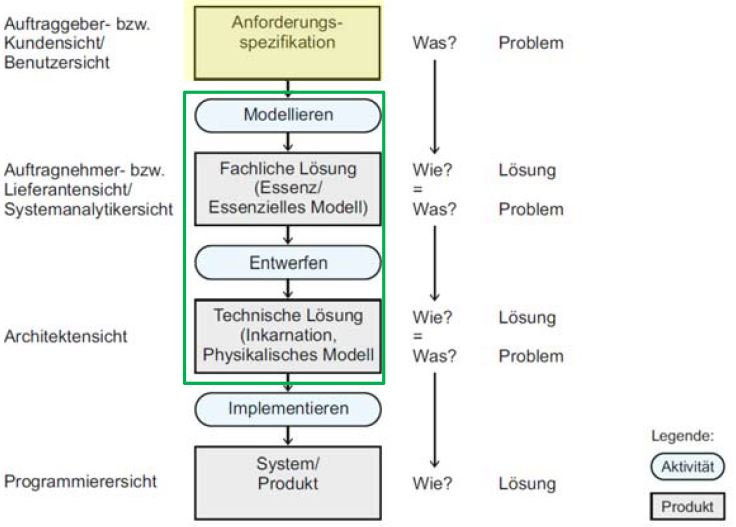
\includegraphics{Figures/Probleml}}
\end{minipage}
\begin{minipage}{7cm}
	Elemente davon sind: 
	\begin{itemize}
		\item Anforderungen: Pflichtenheft
		\item Fachliche Lösung: OOA-Modell
		\item Technische Lösung: OOD-Modell
	\end{itemize}
Das OOA- und OOD-Modell sind Thema im Modul OOAD. 
Je weitere im Prozess, desto stärker wird der Lösungsraum eingeschränkt, wobei der Detaillierungsgrad der Lösung zeitgleich steigt. 
\end{minipage}

\subsection{Hauptgründe für einen Projektabbruch} 
- Änderungen der Anforderungen - 33 \% \\
- Mangelnde Einbindung des höheren Managements - 33 \% (Top Mgmt Committment) \\
- Engpass im Budget - 28 \% \\
- Fehlende Projektmanagement-Fähigkeiten - 28\% \\
--> Siehe Bild zu den "Relativen Bugfixing Kosten"

\section{Anforderungen und Anforderungsarten}
Die Anforderungen legen fest, was man (Stakeholder / Auftraggeber) von einem Softwaresystem als Eigenschaft (Visionen, Ziele, Rahmenbedingungen) erwartet. Eigenschaften lassen sich in funktionale und nichtfunktionale Anforderungen unterteilen. 
Die Anforderungsspezifikationen werden bei der Projektausschreibung in Lasten- und 
Pflichtenheft unterteilt. \\
\begin{minipage}{10cm}
	\adjustbox{width=10cm}{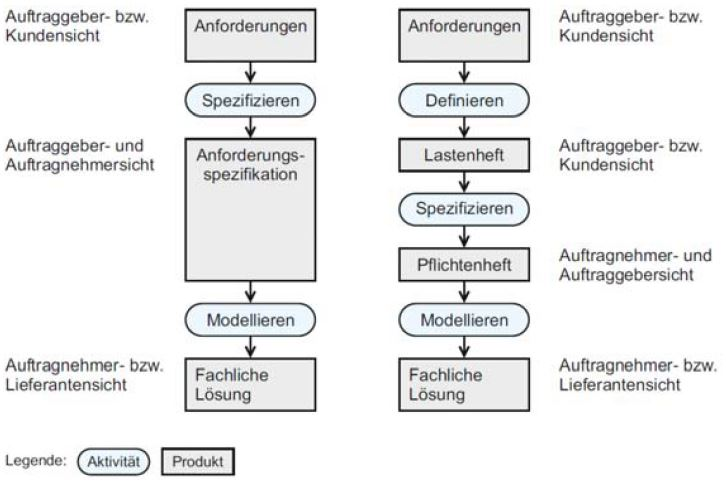
\includegraphics{Figures/anforderungsspezifikation}}
\end{minipage}
\begin{minipage}{7cm}
	\textbf{Lastenheft} \\
	- Zusammenstellung der Anforderungen \\
	- WAS und WOFÜR aus Sicht des Auftraggebers \\
	\textbf{Pflichtenheft} \\
	- Beschreibung der Realisierung der Anforderungen vom Lastenheft \\
	\textbf{Vision} \\
	- Beschreibt eine realitätsnahe Vorstellung der gewünschten Zukunft \\
	- Sie beschreibt, was erreicht werden soll, sagt aber nicht wie \\
\end{minipage}

\textbf{Regeln zur Definition von Zielen:}\\
Ausgehend von einer Vision dienen Ziele dazu, die Vision zu verfeinern und zu operationalisieren.
\begin{enumerate}
	\item Kurz und Prägnant --> Füllwörter vermeiden
	\item Aktivformulierungen verwenden --> Akteur klar benennen
	\item Überprüfbare Ziele formulieren --> Spezifisch
	\item Ziele, die nicht überprüft werden können, nicht verfeinern
	\item Den Mehrwert eines Ziels hervorheben
	\item Das Ziel sollte begründet werden --> Die Zielbegründung führt zur Identifikation weiterer Ziele
	\item Keine Lösungsansätze geben, da sie den Lösungsraum zu früh einschränken würden
\end{enumerate}

\textbf{Rahmenbedingungen} \\
Eine Rahmenbedingung – auch Restriktion genannt – legt organisatorische und/oder technische Restriktionen für das Softwaresystem und/oder den Entwicklungsprozess fest. 
\begin{multicols}{2}
\textbf{Organisatorische Rahmenbedingungen}
\begin{itemize}
	\item Anwendungsbereiche
	\item Zielgruppen
	\item Betriebsbedingungen
	\item Technische Rahmenbedingungen
\end{itemize}
\columnbreak
\textbf{Technische Produktumgebungen}
\begin{itemize}
	\item Welche SW / HW Komponenten sind auf der Zielmaschine
	\item Anforderungen an die Entwicklungsumgebung
	\item SW / HW
\end{itemize}
\end{multicols}

\textbf{Kontext und Überblick} \\
\begin{minipage}{10cm}
Festlegung der Einbettung in materielle und immaterielle Umgebung wie Sensoren, Personen, Übertragungsmedien, APIs, Internet zur Ermittlung der Systemgrenze (Use Case Diagramm). 
\end{minipage}
\begin{minipage}{5cm}
	\adjustbox{width=5cm}{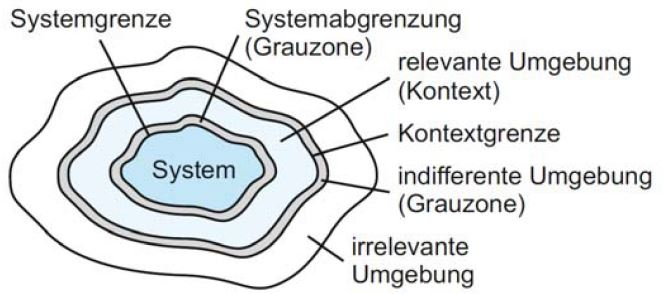
\includegraphics{Figures/kontext}}
\end{minipage}

\textbf{Funktionale \& Nichtfunktionale Anforderungen} \\
\begin{multicols}{2}

\textbf{Funktionale Anforderungen}
\begin{itemize}
	\item das System beschreibende Anforderungen
	\item Statik
	\item Dynamik
	\item Logik
\end{itemize}
\columnbreak
\textbf{Nichtfunktionale Anforderungen}
\begin{itemize}
	\item Qualitätsanforderungen
	\item Genauigkeit, Verfügbarkeit, Zuverlässigkeit
	\item Sicherheit vs. Benutzbarkeit
	\item Speichereffizienz vs. Laufzeiteffizienz
\end{itemize}
\end{multicols}
Nichtfunktionale Anforderungen betreffen mehrere oder alle funktionalen Anforderungen und können sich gegenseitig beeinflussen

\textbf{Natürlichsprachliche Anforderungen} \\
Die Verwendung ist einfach \\
+ flexibel \\
- Synonyme (z.B. City – Innenstadt) und Homonyme (z.B. Bank) führen zu einer lexikalischen Mehrdeutigkeit

Syntaktische Mehrdeutigkeit \\
Die letzten 10 Buchungen und die Stornierungen des Kunden werden im Fenster angezeigt"

Semantische Mehrdeutigkeit \\
"Jeder Sensor ist mit einem Service verbunden" \\

Referentielle Mehrdeutigkeit \\
Beim Login muss zuerst das Benutzerkennzeichen und dann das Passwort eingegeben werden. Ist dies nicht korrekt, schlägt die Anmeldung fehl." \\

Vage Begriffe \\
Der Sensor muss neben der Tür angebracht werden" \\

Sprachliche Anforderungsschablone können verwendet werden.

\section{Anforderungsschablonen}

\begin{figure}[ht]
	\centering
	\adjustbox{width=\textwidth}{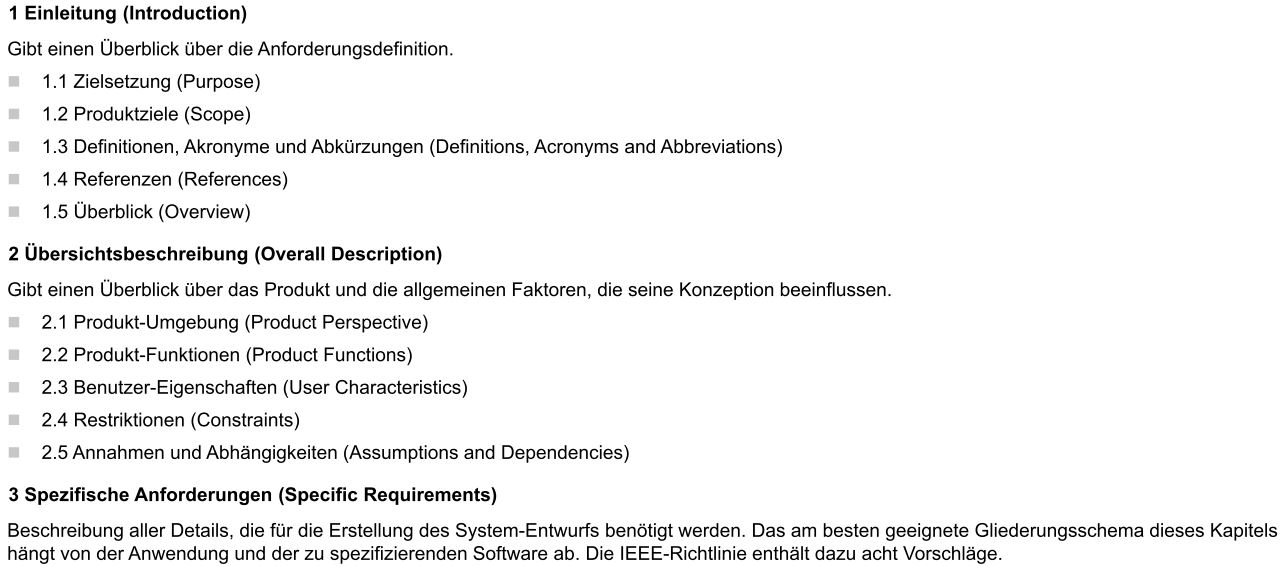
\includegraphics{Figures/ieee-schablone}}
	\caption[]{IEEE Schablone}
\end{figure}
%
%1 Einleitung (Introduction)
%Gibt einen Überblick über die Anforderungsdefinition.
%\begin{itemize}
%	\item 1.1 Zielsetzung (Purpose)
%	\item 1.2 Produktziele (Scope)
%	\item 1.3 Definitionen, Akronyme und Abkürzungen (Definitions, Acronyms and
%\end{itemize}
%
%Abbreviations)
%\begin{itemize}
%\item 1.4 Referenzen (References)
%\item 1.5 Überblick (Overview)
%\item 2 Übersichtsbeschreibung (Overall Description)
%\end{itemize}
%
%Gibt einen Überblick über das Produkt und die allgemeinen Faktoren, die seine Konzeption beeinflussen.
%\begin{itemize}
%\item 2.1 Produkt-Umgebung (Product Perspective)
%\item 2.2 Produkt-Funktionen (Product Functions)
%\item 2.3 Benutzer-Eigenschaften (User Characteristics)
%\item 2.4 Restriktionen (Constraints)
%\item 2.5 Annahmen und Abhängigkeiten (Assumptions and Dependencies)
%\end{itemize}

\textbf{3 Spezifische Anforderungen (Specific Requirements)} \\
Beschreibung aller Details, die für die Erstellung des System-Entwurfs benötigt werden. Das am besten geeignete Gliederungsschema dieses Kapitels 
hängt von der Anwendung und der zu spezifizierenden Software ab. Die IEEE-Richtlinie enthält dazu acht Vorschläge.\\
\begin{itemize}
	\item Externe Schnittstellen-Anforderungen (External Interface Requirements)
	\item Funktionale Anforderungen (Functional Requirements)
	\item Leistungsanforderungen (Performance Requirements)
	\item Entwurfsrestriktionen (Design Constraints)
	\item Eigenschaften des Softwaresystems (Software Systems Attributes)
	\item Andere Anforderungen (Other Requirements)
\end{itemize}

\section{Anforderungen ermitteln und spezifizieren}
\begin{figure}[ht]
	\centering
	\adjustbox{width=9cm}{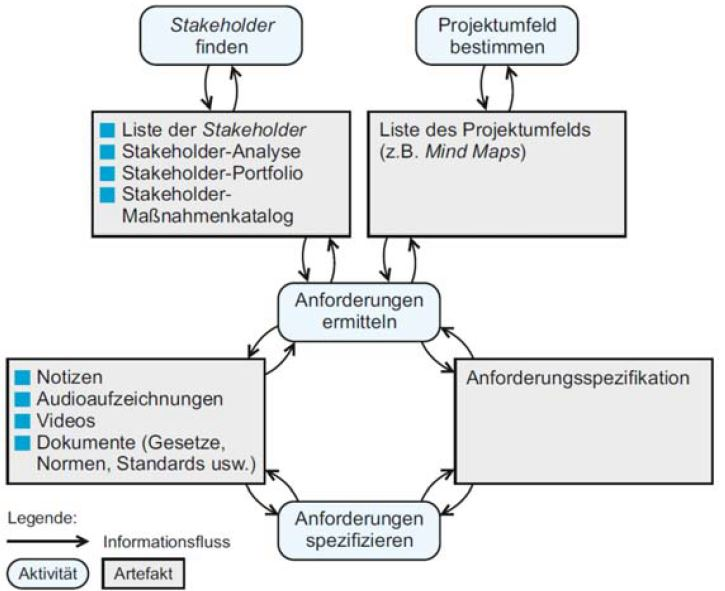
\includegraphics{Figures/ProzesszurAnforderungsdefinition}}
	\caption[]{Prozess zur Anforderungsdefinition}
\end{figure}

\begin{figure}[ht]
	\centering
	\adjustbox{width=\textwidth}{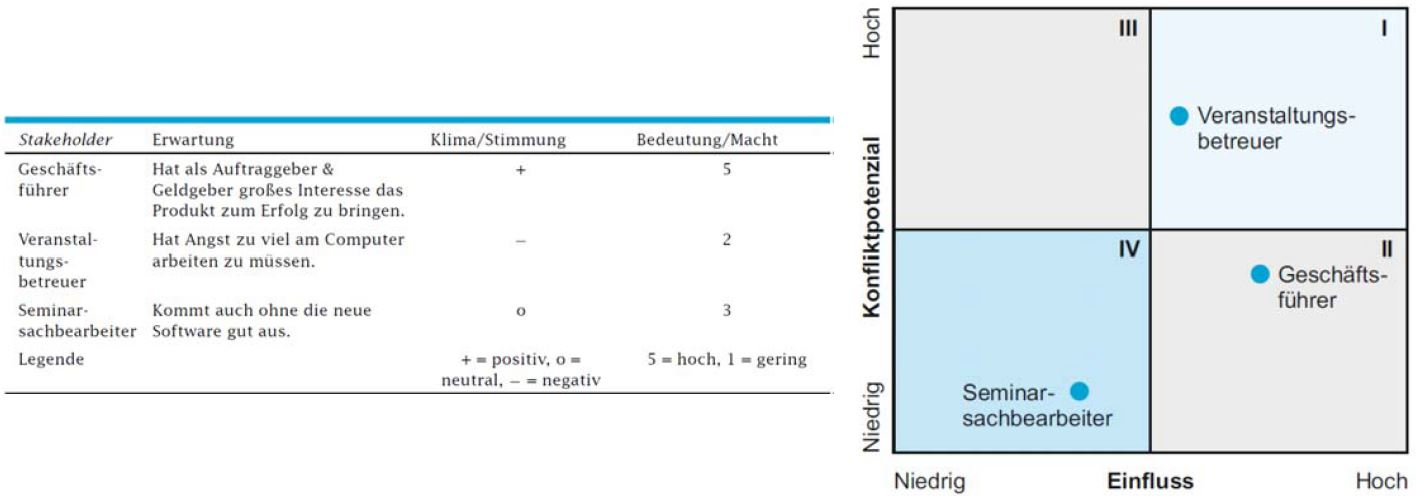
\includegraphics{Figures/Stakeholderportfolio}}
	\caption[]{Stakeholderanalyse \& -portfolio}
\end{figure}

\subsection{Projektumfeld ermitteln}

Es geht darum das Umfeld des Projekts, welche das Projekt wesentlich beeinflussen können zu ermitteln. Das sind meist Vorgaben, Gesetze, Standards, Normen sowie ökologische, ökonomische, gesellschaftliche und kulturelle Einflüsse. 

\subsection{Anforderungen ermitteln}

Die Anforderungen können über Stakeholderbefragungen ermittelt werden. \\
- Erwarten Sie keine präzise Anforderung \\
- Erwarten Sie viel mehr schwammige, unvollständige, widersprüchliche Anforderungen \\
- Überlassen sie die Federführung für die Ermittlung von Anforderungen nicht einem Stakeholder \\

\textbf{Befragungstechniken} \\
- Strukturiertes Interview anhand Anforderungsschablone \\
- Selbstaufschreibung \\
- Stakeholder schreiben Arbeitsabläufe und Wünsche auf \\
- Analyse des Altsystems, falls vorhanden \\
 Die Ergebnisse der Anforderungsermittlung können nun systematisch ausgewertet und schrittweise in die Anforderungsschablone eingetragen werden

\section{Anforderungen priorisieren}

\textbf{Klassifizierung und Priorisierungsmethoden der Anforderungen} \\
-  Nach Kriterium: Häufig wir Notwendigkeit als Kriterium verwendet \\
- Mögliche Unterteilung nach IEEE830, S.13 in essenziell (essential), Bedingt notwendig (conditional), Optional (optional) \\

\textbf{Einige Priorisierungsmethoden} \\
- Ad-hoc Anordnung \\
- Reihenfolge der Anforderungen von Stakeholder oder Gruppe \\
- Top-Ten-Methode \\
- n-Anforderungen werden anhand Kriterium in Rangfolge gebracht
\newpage
\subsection{Kano-Modell}
\begin{multicols}{2}
	\adjustbox{width=6.9cm}{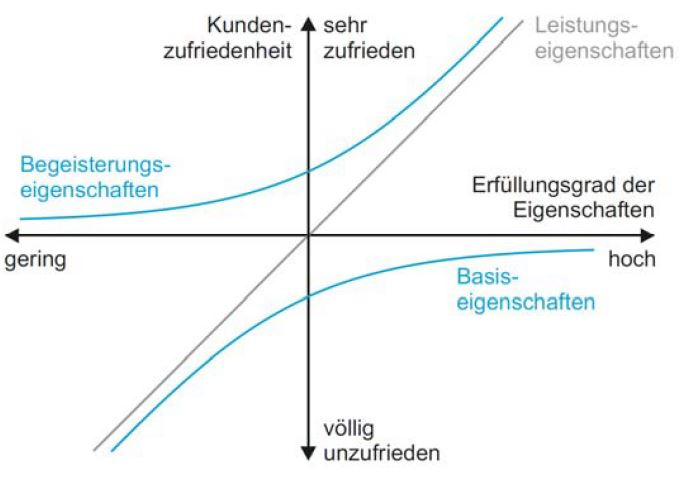
\includegraphics{Figures/kanomodell}} \\
\columnbreak
\\
Kano-Klassifikation \\
- Basiseigenschaft: vom Kunden implizit erwartet \\
- Leistungseigenschaft: vom  Kunden explizit gefordert \\
- Begeisterungseigenschaft: vom Kunden nicht erwartet \\ 
\end{multicols}
Das Kano-Modell kann auch für Anforderungen 
verwendet werden. \\
\begin{figure}[ht]
	\centering
	\adjustbox{width=\textwidth}{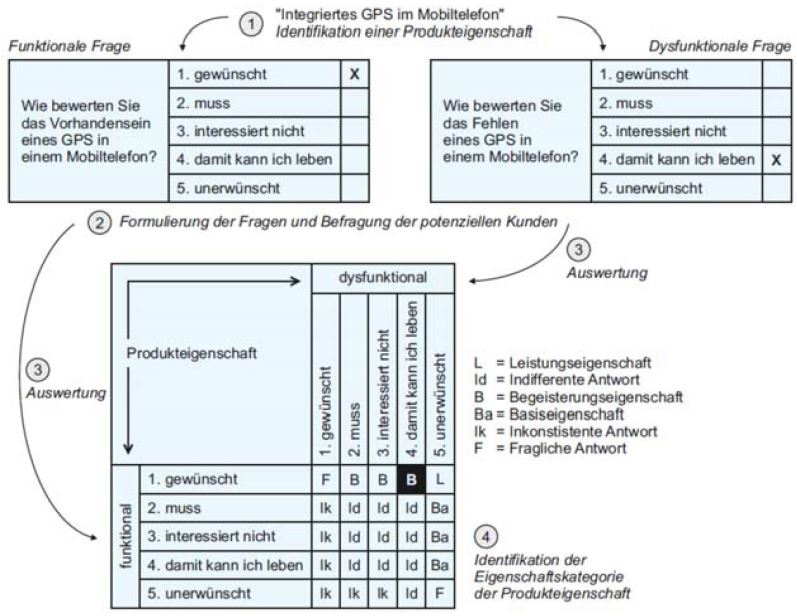
\includegraphics{Figures/kanomodell2}}
	\caption[]{Prozess zur Anforderungsdefinition}
\end{figure}